%\title{Retrieving useful signal using local similarity in random noise attenuation}
\title{EMD-seislet transform}
\author{Yangkang Chen and Sergey Fomel}

\lefthead{Chen and Fomel}
\righthead{EMD-seislet transform}
\footer{TCCS-10}
\maketitle


\begin{abstract}
The seislet transform uses a prediction operator which is connected to the local slope or frequency of seismic events. % for the construction of forward transform following the lifting algorithm. The estimation of local slope directly affect the compression performance of the seislet transform. 
In this paper, we propose combining 1D non-stationary seislet transform with empirical mode decomposition (EMD) in the $f-x$ domain. We use EMD to decompose data into smoothly variable frequency components for the following 1D seislet transform. The resultant representation shows remarkable sparsity. %Because of the empirical property of the new transform, we name the transform as the empirical seislet transform, or Eseielet. 
We introduce the detailed algorithm and use one field example to demonstrate the application of the new seislet transform for sparsity-promoting seismic data processing.
\end{abstract}

\section{Introduction}
Sparse approximation aims at extracting the most important information of the given data by a linear combination of pre-specified atom signals with sparse linear coefficients. Sparse approximation theory has been a rapidly evolving field in digital image analysis, since many state-of-the-art signal and image processing tasks have been successfully handled with the concept of sparsity, including image inpainting and restoration \cite[]{elad2005,mairal2008,mairal2009,jianfeng2013}, image denoising \cite[]{protter2009,jianfeng2013}, data compression \cite[]{bryt2008}, blind source separation \cite[]{zib2001}, etc.

Over the past several decades, different types of sparse transforms have been explored for seismic data processing applications, and promising results have been reported. \cite{luoyi1992} applied a wavepacket transform to seismic data compression. \cite{zhangr2003} developed a type of wavelet frame that takes into account the characteristics of seismic data both in time and space for denoising applications. \cite{ioup1998} applied wavelet transform to both random noise removal and data compression with soft thresholding in the wavelet domain. \cite{du2000} applied multi-resolution property of wavelet transform to attenuate tube waves. \cite{jafarpour2009} used a discrete cosine transform (DCT) to obtain sparse representations of fields with distinct geologic features and improve the solutions to traditional geophysical estimation problems. A number of researchers have also reported successful applications of the curvelet transform \cite[]{candes20061} in different seismic data processing tasks thanks to the multi-scale and sparse property of the curvelet domain \cite[]{hennenfent2006,deli2008}. %Recently, Shearlet transfom has also been used to attenuate random noise.%, such as facies reconstruction from both scattered point measurements and areal observations, crosswell traveltime tomography and porosity estimation in a typical multiunit oil field,  by forming a sparsity-promoting regularization.

\cite{fomel2010seislet} introduced a data-adaptive sparsity promoting transform, called the \emph{seislet} transform. Following the lifting scheme used in the construction of second-generation digital wavelets \cite[]{sweldens1995}, the seislet transform utilizes the spatial predictability property of seismic data to construct the predictive operator. \cite{fomel2010seislet} used plane-wave construction (PWD) to aid the prediction process. Instead of using PWD, \cite{liuyang2010} used differential offset continuation (OC) to construct seislet transform for pre-stack reflection data. OC-seislet transform can obtain better sparsity for conflicting-dip pre-stack seismic data in that OC seislet uses offset continuation \cite[]{fomel2003} instead of local slopes to connect different common offset gathers. %however, at the expense of much higher computational cost. 
In order to relieve the dependence of seislet transform on local slope estimation, \cite{liuyang2013} and \cite{liuyang2015} proposed a velocity-dependent (VD) seislet transform based on conventional velocity analysis. The seislet transform has also found a recent application in simultaneous-source separation \cite[]{yangkang20142}. Instead of using a single slope or frequency map to sparsify the seismic data, \cite{fomel2010seislet} proposed to apply several seislet transforms with smoothly variable slopes or frequencies, which are referred to as seislet frames.

Empirical mode decomposition (EMD) is a recently popular signal processing method \cite[]{huangemd}, which was proposed to prepare a stable input for the Hilbert transform.  The essence of EMD is to stabilize a highly non-stationary signal by decomposing it into smoothly variable frequency components, which are called  intrinsic mode functions (IMF). EMD has found many successful applications in seismic data processing, such as time-frequency analysis \cite[]{jiajun2013} and noise attenuation \cite[]{bekara2009,yangkang20141,yangkang2014emdsum,yangkang2015}. 

%The 2D seislet transform refers to transform the seismic record in the spatial direction following the local slope. For most seismic record, the seislet transform can obtain very compressed transform domain provided that an accurate local slope estimation is given. However, in most situations, the estimation of the local slope can not be easily obtained, which affect greatly the compression performances.  
In this paper, we propose to use EMD to create sparse transforms for representing seismic data. %also following the local slope but without calculating slope estimation. 
We first transform the input seismic data from $t-x$ domain to $f-x$ domain, then apply EMD to each frequency slice to decompose input data into smoothly variable frequency components. Next, 1D non-stationary seislet transform is applied independently to each component. We evaluate the sparsity of the new representation (EMD-seislet transform) and apply it to noise attenuation of a seismic image.
%. Because the seismic data is highly non-stationary along the spatial direction, we use EMD to prepare the stable input with  Since EMD can empirically separate different wavenumber components, which corresponds to different slope components, thus it makes the new sparse transform free of slope estimation. %Because of the empirical property of the transform, we name it as empirical seislet transform, or EMD-seislet transform. The inverse EMD-seislet transform follows the inverse of each of the aforementioned procedures. 



%The aim of empirical mode decomposition (EMD) is to empirically decompose a non-stationary signal into a finite set of stationary sub-signals, which are termed as intrinsic mode functions (IMF) and are considered to have smoothly varying frequencies \cite[]{huangemd}. %The IMFs satisfy two conditions: (1) in the whole data set, the number of extrema and the number of zero crossings must either \new{be} equal or differ at most by one; and (2) at any point, the mean value of the envelope\new{s} defined by the local maxima and \old{the envelope defined by} the local minima is \new{reasonably close to} zero \cite[]{emd}.

\section{Method}
\subsection{Empirical mode decomposition}
The process of EMD has the following simple expression: 
\begin{equation}
\label{eq:emd}
s(t)=\sum_{n=1}^{N}c_n(t)+r(t),
\end{equation}
where $s(t)$ is the original non-stationary signal, $c_n(t)$ ($n=1,2,\cdots,N$) denotes each separated IMF, $N$ denotes the number of separated IMF, and $r(t)$ denotes the residual after EMD.

The process of EMD is to gradually remove the stable oscillations embedded in the original signal to arrive at a monotonic and smooth residual or trend at last. A special property of EMD is that the IMFs represent different oscillations embedded in the data, where the oscillating frequency for each sub-signal $c_n(t)$ decreases with IMF order increasing \cite[]{huangemd,yangkang20141}. %Ideally, each sub-signal will contain oscillating components with relatively constant frequency, as demonstrated in \cite[]{yangkang20141}.

More explicit approaches to decomposing data into spectral components were proposed by recently \cite{fomel20132} and \cite{hou2}.

\subsection{1D seislet transform}
The seislet transform can be constructed by multiscale prediction of the odd components from the even components:
\begin{align}
\label{eq:r}
\mathbf{r}&=\mathbf{o}-\mathbf{P}(\mathbf{e}), \\
\label{eq:e}
\mathbf{c}&=\mathbf{e}+\mathbf{U}(\mathbf{r}).
\end{align}
$\mathbf{P}$ denotes the prediction operator and $\mathbf{U}$ denotes the updating operator at a particular scale. The inverse seislet transform follows the inverse process of equations \ref{eq:r} and \ref{eq:e} continuing from large to small scale. The difference between 1D seislet transform and 1D wavelet transform is whether the prediction is modulated by an appropriate frequency. In the simplest case of Haar transform, the Z-transform domain prediction filter for the Haar wavelet transform is 
\begin{equation}
\label{eq:haar}
P(Z)=Z,
\end{equation}
and the Z-transform domain Haar prediction filter for wavelet transform is 
\begin{equation}
\label{eq:haaru}
U(Z)=Z/2.
\end{equation}

However, for seislet transform,
\begin{align}
\label{eq:haarseis}
P(Z)&=Z/Z_0, \\
\label{eq:haarseisu}
U(Z)&=1/2(Z/Z_0).
\end{align}
where $Z_0=e^{i\omega_0\Delta t}$. The prediction filter \ref{eq:haarseis} can perfectly characterizes a sinusoid with $\omega_0$ circular frequency sampled on a $\Delta t$ grid.
Analogously, the prediction filter for biorthogonal 2/2 transform can be expressed as:
\begin{equation}
\label{eq:linearseis0}
P(Z)=1/2(Z/Z_0+Z_0/Z),
\end{equation}
and its corresponding updating operator is
\begin{equation}
\label{eq:uplinearseis0}
U(Z)=1/4(Z/Z_0+Z_0/Z).
\end{equation}

%\subsection{1D non-stationary seislet transform}
%Let us take the prediction filter \ref{eq:linearseis0} as an example.
When a 1D signal has a constant circular frequency, the prediction filter \ref{eq:haarseis} can characterize a sinusoidal signal. When the 1D signal contains a sinusoid with a variable frequency, or in other words, is non-stationary, we can replace $Z_0$ with $Z_t$,  $Z_t=e^{i\omega(t)\Delta t}$ denotes the frequency modulation at time $t$.%modify equation \ref{eq:linearseis0} to the following form
%\begin{equation}
%\label{eq:linearseis}
%P(Z)_t = 1/2(Z/Z_t + Z_t/Z),
%\end{equation}
%in order to best characterize the non-stationary signal. $P(Z)_t$ denotes the prediction filter at time $t$, and $Z_t=e^{i\omega(t)\Delta t}$ denotes the frequency modulation at time $t$.
%In the physical domain, the linear prediction and updating operators can be expressed as:
%\begin{align}
%\label{eq:linearseis-phy}
%P(e)_t&=(S^{(+)}(e_{k-1}) + S^{(-)}(e_t))/2,\\
%\label{eq:linearseisu-phy}
%U(r)_t&=(S^{(+)}(r_{k-1}) + S^{(-)}(r_t))/4,
%\end{align}
%where $S_t^{(+)}$ and $S_t^{(-)}$ are operators that predict an element from its left and right neighbors by modulating each element according to their local frequency $\omega(t)$.

Figure \ref{fig:non-comp2} shows a comparison between wavelet transform and 1D stationary and non-stationary seislet transforms in compressing a 1D signal with smoothly variable frequency components. The frequency ranges from 250 to 186 Hz. Both the wavelet transform and stationary seislet transform fail to compress the signal well while the non-stationary seislet transform obtains a perfectly sparse representation.

\inputdir{nonseis}
\plot{non-comp2}{width=\columnwidth}{Demonstration of 1D non-stationary seislet transform for non-stationary signal. Upper: non-stationary chirp signal, frequency ranges from 250 to 186 Hz. Upper middle: compressed using 1D wavelet transform. Down middle: compressed using 1D stationary seislet transform with the frequency of 250 Hz. Down: compressed using 1D non-stationary seislet transform.}


\subsection{Estimating local frequency by complex non-stationary autoregression}
According to the autoregressive spectral analysis theory \cite[]{marple}, a complex time series that has a constant frequency component is predictable by a two-point prediction-error filter $(1,-e^{i\omega_0\Delta t})$. Suppose a complex time series is $d(t)$. In Z-transform notation, the two-point prediction-error filter can be expressed as:
\begin{equation}
\label{eq:twopre}
F(Z)=1-Z/Z_0.
\end{equation} 
We assume a 1D time series have a smoothly variable frequency component, then the 1D time series can be locally predicted using different local two-point prediction-error filters $(1,-e^{i\omega(t)\Delta t})$:
\begin{equation}
\label{eq:localpre}
d(t)=e^{i\omega(t)\Delta t}d(t-\Delta t).
\end{equation}

In order to estimate $\omega(t)$ using equation \ref{eq:localpre}, we 
%need to first minimize the least-squares misfit of the true and predicted time series with a local-smoothness constraint:
%\begin{equation}
%\label{eq:mini}
%\min_{\mathbf{a}} \parallel \mathbf{d} - \mathbf{D} \mathbf{a} \parallel_2^2 + \mathbf{R}(\mathbf{a}),
%\end{equation}
%where $\mathbf{d}$ and $\mathbf{a}$ are vector composed of the entries $d(t)$ and $a(t)$, respectively, and $a(t)=e^{i\omega_{t}\Delta t}$. $\mathbf{D}$ is a diagonal matrix composed of the entries $d(t-\Delta t)$. $\mathbf{R}$ denotes the local-smoothness constraint. We 
use non-stationary auto-regression \cite[]{fomel20095,fomel20132}.
%Equation \ref{eq:mini} can be solved using shaping regularization \cite[]{fomel2007shape}:
%\begin{equation}
%\hat{\mathbf{a}} = [\lambda^2\mathbf{I}+\mathcal{T}(\mathbf{D}^T\mathbf{D}-\lambda^2\mathbf{I})]^{-1}\mathcal{T}\mathbf{D}^T\mathbf{d},
%\end{equation}
%where $\mathcal{T}$ is a triangle smoothing operator and $\lambda$ is a scaling parameter that controls the physical dimensionality and enables fast convergence \cite{fomel2007localattr}. $\lambda$ can be chosen as the least-squares norm of $\mathbf{D}$.

%After the filter coefficient $a(t)$ is obtained, we can straightforwardly calculate the local circular frequency $\omega(t)$ by:
%\begin{equation}
%\label{eq:circ}
%\omega(t) = Re\left[\frac{\mbox{arg}(a(t))}{\Delta t}\right].
%\end{equation}

%\begin{figure*}[ht!]
%  \centering
%  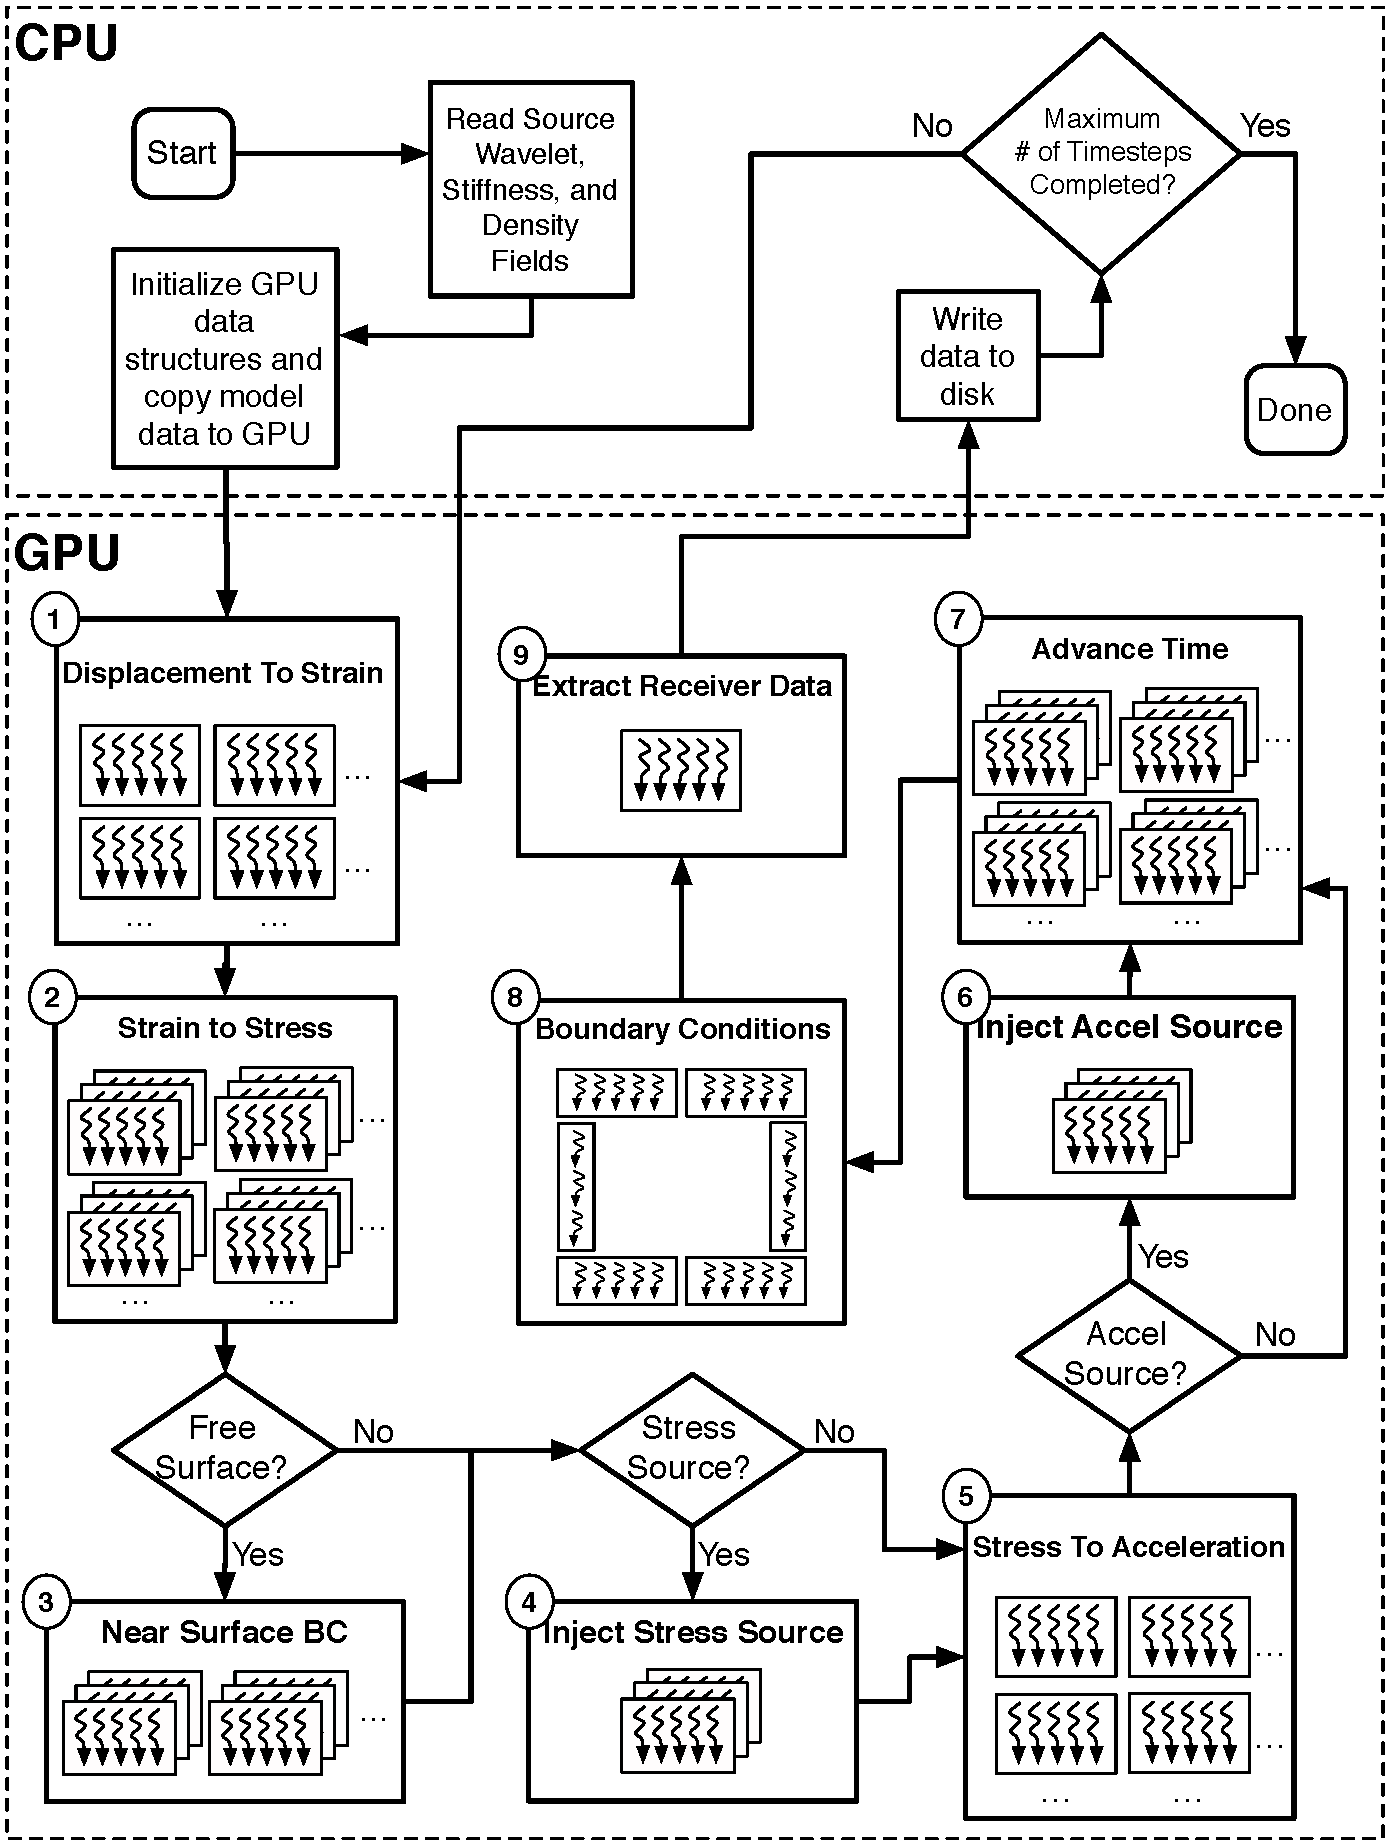
\includegraphics[width=0.7\textwidth]{Fig/flow}
%   \caption{Workflow of EMD-seislet transform.}
%    \label{fig:flow}
%\end{figure*}

\subsection{Preparing smoothly variable frequency components by EMD}

\inputdir{demo2}
\multiplot{2}{demo,demo-fz}{width=0.45\textwidth}{(a) Synthetic example with hyperbolic events. (b) $f-x$ spectrum of (a).}

\inputdir{demo4}
\multiplot{9}{demo-f1z-0,demo-f1z-seis-0,demo-dip1-0,demo-f2z-0,demo-f2z-seis-0,demo-dip2-0,demo-f3z-0,demo-f3z-seis-0,demo-dip3-0}{width=0.29\textwidth}{A demonstration of the EMD-seislet transform. The left column shows the decomposed $f-x$ domain spectrum using EMD. The middle column shows the compressed $f-x$ domain using 1D non-stationary seislet transform. The right column shows the reconstructed $t-x$ domain data corresponding to different components.}




The aforementioned 1D non-stationary seislet transform adapts to 1D signals that have smoothly variable frequency components since its compression performance is controlled by the predicting and updating procedures between the series elements according to a locally smooth modulation frequency. Correspondingly, when calculating the local frequency, we also assume the 1D signal to have smoothly variable frequency components. Figure \ref{fig:demo-fs-3} shows a demonstration for preparing smoothly variable frequency components for each frequency slices using EMD in the $f-x$ domain.




%For single plane-wave seismic profiles, each frequency slice in the frequency-space domain can be considered as a locally stationary 1D signal. However, when the plane-wave components are many, which also refers to a large number of dipping components, the frequency slice in the frequency-space domain is considered as highly non-stationary. In order to prepare a locally stationary 1D signal in each frequency slice, we propose to apply EMD to each frequency slice and obtain several IMFs. Each IMF can be seen as locally stationary 1D signal, and thus can be compressed using the 1D non-stationary seislet transform. A special property of the EMD is its highly adaptive decomposition. We do not need to specify any parameter except for the number of IMFs and thus we can operate it very conveniently. 

We call the combined FFT-EMD-seislet workflow the \emph{EMD-seislet} transform. Figures \ref{fig:demo,demo-fz} and \ref{fig:demo-f1z-0,demo-f1z-seis-0,demo-dip1-0,demo-f2z-0,demo-f2z-seis-0,demo-dip2-0,demo-f3z-0,demo-f3z-seis-0,demo-dip3-0} provide a detailed demonstration of the procedures involved in the EMD-seislet transform construction. Figure \ref{fig:demo} shows a synthetic data with hyperbolic events. Figure \ref{fig:demo-fz} shows the $f-x$ spectrum of the synthetic data. We can observe that each frequency slice in the $f-x$ domain is highly non-stationary. After EMD decomposition, the three decomposed $f-x$ domain components are shown in the left column of Figure \ref{fig:demo-f1z-0,demo-f1z-seis-0,demo-dip1-0,demo-f2z-0,demo-f2z-seis-0,demo-dip2-0,demo-f3z-0,demo-f3z-seis-0,demo-dip3-0}. Each component now has smoothly non-stationary frequency slices. After 1D non-stationary seislet transforms, the three $f-x$ domain components become highly compressed. The middle column in Figure \ref{fig:demo-f1z-0,demo-f1z-seis-0,demo-dip1-0,demo-f2z-0,demo-f2z-seis-0,demo-dip2-0,demo-f3z-0,demo-f3z-seis-0,demo-dip3-0} shows the compressed $f-x$ domain using the 1D non-stationary seislet transform. The right column in Figure \ref{fig:demo-f1z-0,demo-f1z-seis-0,demo-dip1-0,demo-f2z-0,demo-f2z-seis-0,demo-dip2-0,demo-f3z-0,demo-f3z-seis-0,demo-dip3-0} shows the reconstructed $t-x$ domain data from the decomposed and compressed components in the middle column. The three decomposed components correspond to different parts of the input signal.% three different slopes. % The EMD-seislet transform domain appears sparse.

In order to compare the sparsity in compressing seismic data, we plot the reconstruction error curves with respect to the number of selected largest coefficients. The reconstruction error is defined as $E=\parallel\mathbf{d}-\mathbf{Am}_N\parallel_2^2$, where $\mathbf{m}_N$ denotes the largest $N$ coefficients in the transform domain. The faster the curve decays, the sparser the corresponding transform domain will be. As shown in Figure \ref{fig:sparse}, the EMD-seislet appears to be the sparsest compared with the PWD-seislet transform, wavelet transform, and Fourier transform.


\inputdir{demo2}
\plot{demo-fs-3}{width=0.8\columnwidth}{Demonstration of preparing the smoothly variable frequency components by EMD for the 15 Hz slice of the synthetic data in Figure \ref{fig:demo}.}

%\begin{figure}[htb!]
%  \centering
%  \subfigure[]{\includegraphics[width=0.31\columnwidth,height=0.45\columnwidth]{synth3/Fig/hyper}
%    \label{fig:hyper}}
%  \subfigure[]{\includegraphics[width=0.31\columnwidth,height=0.45\columnwidth]{synth3/Fig/hyper-recon}
%    \label{fig:hyper-recon}}
%  \subfigure[]{\includegraphics[width=0.31\columnwidth,height=0.45\columnwidth]{synth3/Fig/hyper-dif}
%    \label{fig:hyper-dif}} 
%   \caption{(a) Synthetic example. (b) Forward and inverse EMD-seislet transform reconstructed data. (c) Reconstruction error.}
%       \label{fig:hyper,hyper-recon,hyper-dif}
%\end{figure}
%\begin{figure}[htb!]
%  \centering
%  \includegraphics[width=0.6\columnwidth]{synth/Fig/hyper}
%    \label{fig:sigcoef}
%   \caption{Hyperbolic synthetic example}
%\end{figure}

\inputdir{sparse}
\plot{sparse}{width=\columnwidth}{Sparsity comparison. $E=\parallel\mathbf{d}-\mathbf{Am}_N\parallel_2^2$ denotes the reconstruction error with the largest $N$ coefficients in the transform domain.}

\section{Examples}
We use a field data example shown in Figure \ref{fig:real} to demonstrate the performance of the proposed EMD-seislet in attenuating random noise. Figure \ref{fig:real-eseist-g} shows the denoised result by thresholding in the EMD-seislet transform domain. Figure \ref{fig:real-eseist-dif-g} shows the remove noise section using EMD-seislet thresholding. 2\% of EMD-seislet coefficients were retained. Despite the complicated structures of the seismic image, the proposed approach obtains a successful denoising performance.

% From the comparison in Figures \ref{fig:real-eseist-0,real-eseist-dif-g,real-seist-0,real-seist-dif-g,real-fx-0,real-fx-dif-g} and \ref{fig:real-z,real-eseist-z,real-seist-z,real-fx-z}, the proposed approach obtains the best result, while seislet thresholding is over-smoothing and FX decon harms some of the signal energy.

\section{Conclusion}
We have proposed a novel approach to sparsifing seismic data: EMD-seislet transform. The approach relies on the ability of empirical mode decomposition (EMD) in the $f-x$ domain to provide smoothly non-stationary data, which we use in the following 1D non-stationary seislet transform. When applied to seismic data with multiple conflicting slopes, EMD-seislet is remarkably sparse. A field data example shows an excellent performance of EMD-seislet transform in attenuating random noise.


%\begin{figure}[htb!]
%  \centering
%  \includegraphics[width=\columnwidth]{synth3/Fig/sigcoef}
%    \label{fig:sigcoef}
%   \caption{Sparsity comparison.}
%\end{figure}

%\begin{figure}[htb!]
%  \centering
%  \subfigure[]{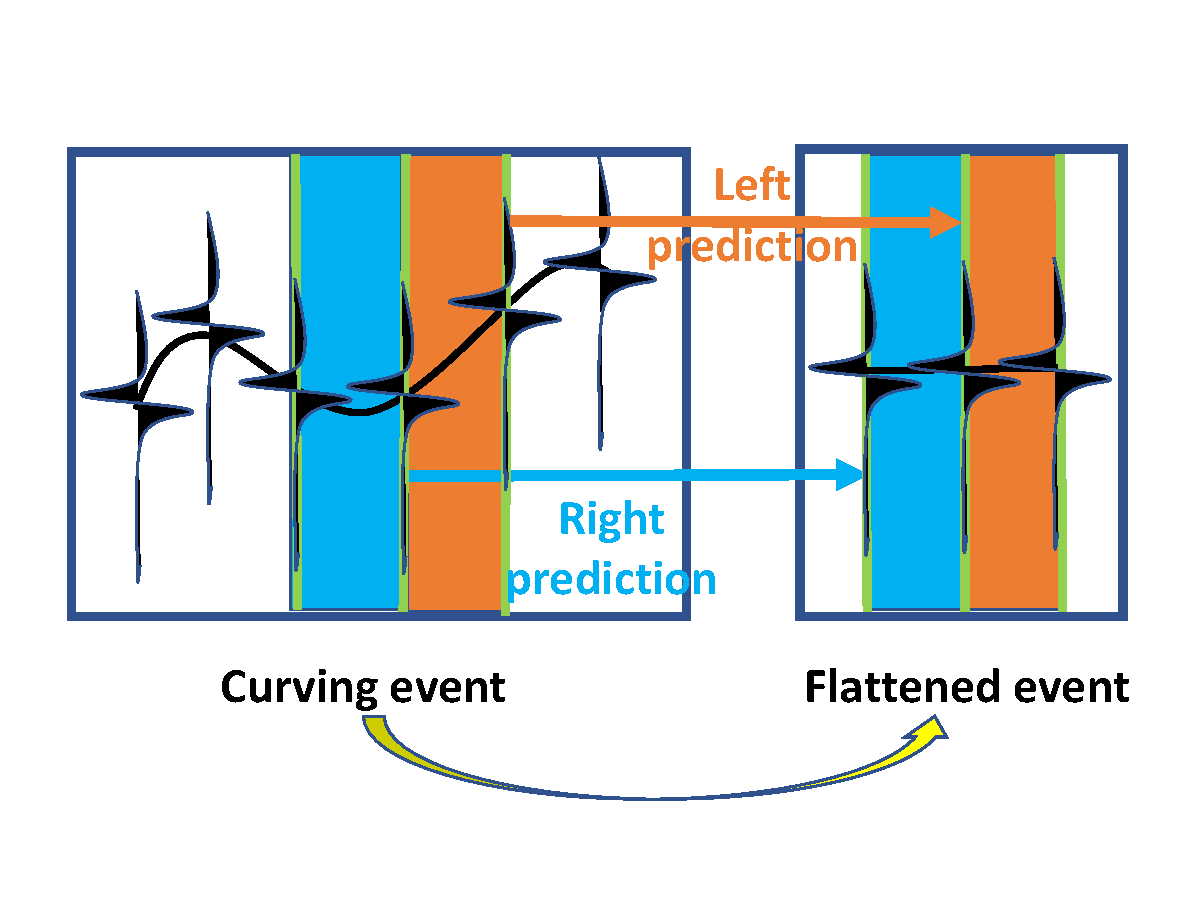
\includegraphics[width=0.45\columnwidth,height=0.5\columnwidth]{demo/Fig/demo}
%    \label{fig:demo}}
%  \subfigure[]{\includegraphics[width=0.45\columnwidth,height=0.5\columnwidth]{demo/Fig/demo-f}
%    \label{fig:demo-f}}
%  \subfigure[]{\includegraphics[width=0.45\columnwidth,height=0.5\columnwidth]{demo/Fig/demo-femd3d}
%    \label{fig:demo-femd3d}} 
%  \subfigure[]{\includegraphics[width=0.45\columnwidth,height=0.5\columnwidth]{demo/Fig/demo-feseis3d}
%    \label{fig:demo-feseis3d}}     
%   \caption{Demonstration of the empirical seislet transform process. (a) Seismic records in $t-x$ domain. (b) Seismic records in $f-x$ domain. (c) EMD decomposed data in $f-x-IMF$ domain. (d) Seislet transformed data in $f-s-IMF$ domain.}
%      \label{fig:demo,demo-f,demo-femd3d,demo-feseis3d}
%\end{figure}


%\begin{figure*}[ht!]
%  \centering
%  \subfigure[]{\includegraphics[width=0.31\textwidth,height=0.5\textwidth]{synth3/Fig/hyper-noisy}
%    \label{fig:hyper-noisy}}
%  \subfigure[]{\includegraphics[width=0.31\textwidth,height=0.5\textwidth]{synth3/Fig/hyper-eseis}
%   \label{fig:hyper-eseis}}
%  \subfigure[]{\includegraphics[width=0.31\textwidth,height=0.5\textwidth]{synth3/Fig/hyper-noise}
%    \label{fig:hyper-noise}} 
%   \caption{Denoising test. (a) Noisy data. (b) Denoised data using EMD-seislet domain thresholding. (c) Noise section.}
%      \label{fig:hyper-noisy,hyper-eseis,hyper-noise}
%\end{figure*}

%\begin{figure*}[ht!]
%  \centering
%  \subfigure[]{\includegraphics[width=0.31\textwidth,height=0.5\textwidth]{inter2/Fig/interp2-zero}
%    \label{fig:interp2-zero}}
%  \subfigure[]{\includegraphics[width=0.31\textwidth,height=0.5\textwidth]{inter2/Fig/interp2-recon}
%    \label{fig:interp2-recon}}
%  \subfigure[]{\includegraphics[width=0.31\textwidth,height=0.5\textwidth]{inter2/Fig/interp2-dif}
%    \label{fig:interp2-dif}} 
%   \caption{Interpolation test. (a) Decimated data. (b) Reconstructed data. (c) Interpolated traces.}
%     \label{fig:interp2-zero,interp2-recon,interp2-dif}
%\end{figure*}



%\inputdir{field}
%\plot{real-0}{width=0.4\textwidth,height=0.25\textwidth}{Seismic image from \cite[]{yangkang2015dsd}.}





\inputdir{field}
\multiplot{3}{real,real-eseist-g,real-eseist-dif-g}{width=0.6\textwidth}{Denoising test. (a) Seismic image from \cite{yangkang2015dsd}. (b) Denoised data using EMD-seislet domain thresholding. (b) Noise section. }
%\begin{figure}[htb!]
%  \centering
%  \subfigure[]{\includegraphics[width=0.22\textwidth,height=0.25\textwidth]{field/Fig/real-z}
%    \label{fig:interp2-zero}}
%  \subfigure[]{\includegraphics[width=0.22\textwidth,height=0.25\textwidth]{field/Fig/real-eseist-z}
%    \label{fig:interp2-recon}}
%  \subfigure[]{\includegraphics[width=0.22\textwidth,height=0.25\textwidth]{field/Fig/real-seist-z}
%    \label{fig:interp2-zero}}
%  \subfigure[]{\includegraphics[width=0.22\textwidth,height=0.25\textwidth]{field/Fig/real-fx-z}
%    \label{fig:interp2-recon}}
%   \caption{Zoomed denoised sections of (a) original noisy data, (b) using EMD-seislet domain thresholding, (c) using seislet domain thresholding, (c) using FX decon.}
%     \label{fig:real-z,real-eseist-z,real-seist-z,real-fx-z}
%\end{figure}


%\newpage
%\onecolumn
\bibliographystyle{seg}
\bibliography{eseis}

























